\documentclass[a4paper,oneside,article,11pt]{memoir}
\usepackage{changepage}
\usepackage[english]{babel}
\usepackage[utf8]{inputenc}
\usepackage{amsmath,amssymb,amsthm}

\newtheorem*{toprove}{At bevise}
\newtheorem{mydef}{Definition}

% This font looks so good.
\usepackage[sc]{mathpazo}
\usepackage{fancybox}
% Typesetting pseudo-code
\usepackage{algorithm}
\usepackage{algorithmic}
\usepackage{multirow}
% Code comments like [CLRS]
\renewcommand{\algorithmiccomment}[1]{\makebox[5cm][l]{$\triangleright$ \textit{#1}}}
\usepackage{framed,graphicx,xcolor}
\usepackage{listings}
\usepackage{hyperref}

\usepackage[font={small,it}]{caption}

% Relative references
\usepackage{varioref}

\usepackage{tikz}

\bibliographystyle{plain}

\title{Bioinformatics - Tree Comparison \\ Project 2}
\author{Peter Gabrielsen 20114179\\
Christoffer Hansen 20114637}
\newcounter{qcounter}

\makeatletter
\newenvironment{CenteredBox}{% 
\begin{Sbox}}{% Save the content in a box
\end{Sbox}\centerline{\parbox{\wd\@Sbox}{\TheSbox}}}% And output it centered
\makeatother

\begin{document}

\maketitle

\chapter*{Introduction}
%A short status of your work. Does everything work as expected, or are there any problems or unsolved issues.
In this project we are going to implement Saitou and Nei's algorithm for Neighbor joining. The aim of the project will be to make it run as fast as possible using different techniques and then compare our fastest implementation against \texttt{RapidNJ} and \texttt{QuickTree}.
Our implementation works as expected.
\\\\Code can be found at \url{https://github.com/gabet1337/bioinformatics}.

\pagebreak

\chapter*{Implementation}
The implementations is done in \texttt{c++}. 
We implemented two different ideas; one naive with heave parallelization and one using the idea from the RapidNJ paper.

\subsection*{OpenMP version}
This version heavily relies on OpenMP to parallelize the naive version of Saitou-Nei's neighbor joining algorithm. The row sums and finding the minimum element in the N matrix is parallelized using OpenMP. When we remove columns and rows we just mark it as deleted and when we have deleted 10\% of the entire matrix we garbage collect the deleted rows and columns and globally rebuild the structure. We tried parallelizing the garbage collection but with a decrease in performance.

It compiles using \texttt{make nj} and runs using \texttt{./nj $<$phylib file$>$}.

As seen in~\ref{fig:openmp} our naive implementation with OpenMP parallization runs within a factor of two of QuickTree. These results were found by repeatedly running the programs and average the running time over 10 runs.

\begin{figure}[H]
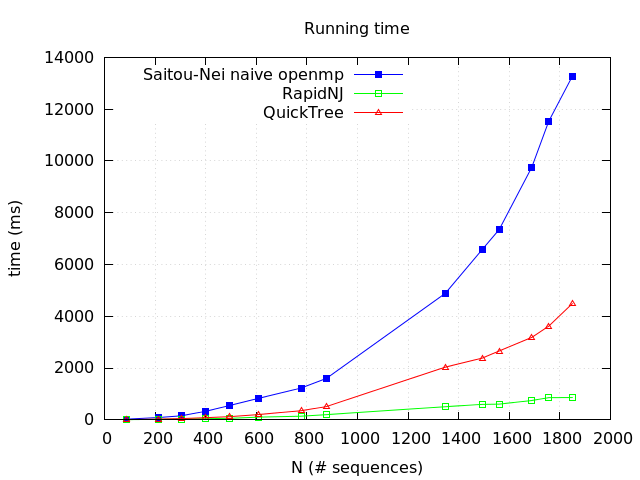
\includegraphics[scale=0.5]{../results/running_time_all.png}
\caption{\label{fig:openmp}Running time of OpenMP version compared to QuickTree and RapidNJ}
\end{figure}

\subsection*{Machine}
Running on an i7-3720QM @ 2.60GHz with 4GB ram in a VMWare Ubuntu 14.04 with kernel 3.16.0-50-generic. Compiled with optimization level 3.

\subsection*{Results }
\begin{figure}[H]
\begin{adjustwidth}{-2.3cm}{}
\begin{tabular}{l|c|c|c|c|c|c|c|c}
						& QT 	& RNJ 	& SN		& QT/SN 		& RNJ/SN & RF(QT,SN)	& RF(RNJ,SN) & RF(RNJ,QT) 	\\\hline
89\_Adeno\_E3\_CR1 		& 5 		& 4 		& 11   	& 0.45	 	& 0.36	 & 18		& 34			 & 30 			\\\hline
214\_Arena\_glycoprot 	& 19 	& 12 	& 69   	& 0.27 		& 0.27	 & 36		& 50			 & 56 			\\\hline
304\_A1\_Propeptide 		& 38 	& 20 	& 98   	& 0.39 		& 0.20	 & 38		& 74			 & 78 			\\\hline
401\_DDE 				& 66 	& 35 	& 150  	& 0.44 		& 0.23	 & 20		& 98			 & 98 			\\\hline
494\_Astro\_capsid 		& 96 	& 44 	& 244  	& 0.39 		& 0.18	 & 244		& 530		 & 532 			\\\hline
608\_Gemini\_AL2 		& 161 	& 91 	& 391  	& 0.41	 	& 0.23	 & 16		& 20			 & 20 			\\\hline
777\_Gemini\_V1 			& 288 	& 123 	& 668  	& 0.43 		& 0.18	 & 148		& 480		 & 494 			\\\hline
877\_Glu\_synthase 		& 420 	& 178 	& 893  	& 0.47 		& 0.20	 & 34		& 60			 & 54 			\\\hline
1347\_FAINT 				& 1660 	& 445	& 2570 	& 0.65 		& 0.17	 & 0			& 2			 & 2 			\\\hline
1493\_Fe-ADH 			& 1919 	& 508 	& 3349 	& 0.57 		& 0.15	 & 10		& 88			 & 92 			\\\hline
1560\_Ferritin 			& 2177 	& 534 	& 3803 	& 0.57 		& 0.14	 & 40		& 146		 & 152 			\\\hline
1689\_FGGY\_N 			& 2636 	& 652 	& 4623 	& 0.57 		& 0.14	 & 26		& 104		 & 102 			\\\hline
1756\_FAD\_binding\_3 	& 2981 	& 720 	& 4890 	& 0.61 		& 0.15	 & 40		& 68			 & 76 			\\\hline
1849\_FG-GAP 			& 3536 	& 729 	& 5675 	& 0.62 		& 0.13	 & 132		& 282		 & 280
\end{tabular}
\caption{\label{tab:results}Results of all experiments}
\end{adjustwidth}
\end{figure}

\subsection*{RapidNJ idea}
%TODO Christoffer adds results for his implementation here!


\chapter*{Conclusion}
We were able to come within a factor of $0.6$ of QuickTree while RapidNJ becomes more and more fast compared to our implementation utilizing OpenMP.

\bibliography{references}

\end{document}


